Inspection camera has to measure the bending angle of the bent sheet metal part. \hyperref[acro:KR]{KR1410} brings the bent sheet to the inspection camera. Correct alignment of the bent sheet by the robot is particularly important for inspection. The detection of edges of sheet takes place in the inspection process by the reflection of camera's internal red light around the sheet edges. Since the edges of the sheet could have different surface structure or have impurities over them, angle tolerance needs to be setup for each inspection. Separate job is to be created for each inspection.

\begin{figure}[h]
    \centering
    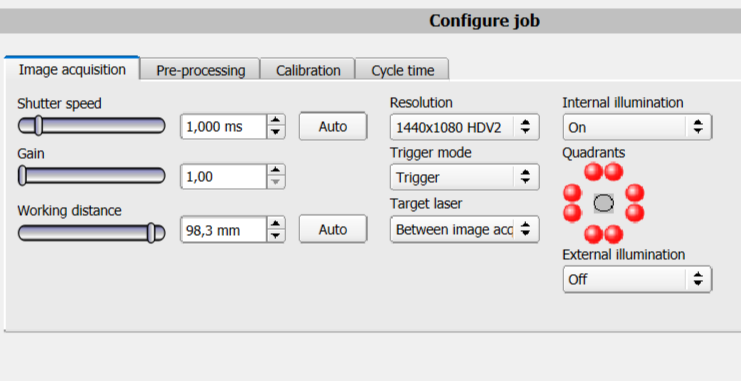
\includegraphics[width=\textwidth]{figures/job-configuration-object.png}
    \caption{Job configuration for the object camera}
    \label{fig:job-configuration-object}
\end{figure}

For the inspection of bent sheet, a job is created with the configuration as shown in figure \ref{fig:job-configuration-object}. A working distance is set in the range of 90 mm to 130 mm for each inspection job. This is the optimum distance for the inspection as the object needs to fully illuminated by the red light. The shutter speed is set to 1.0 ms. This means the camera lens will open only for a duration of 1.0 ms. Thus, only the red light is used to capture the bent sheet image and there is no issue of ambient light. Internal illumination is required in this case.
Only images processing is required by this camera.

\begin{figure}[h]
    \centering
    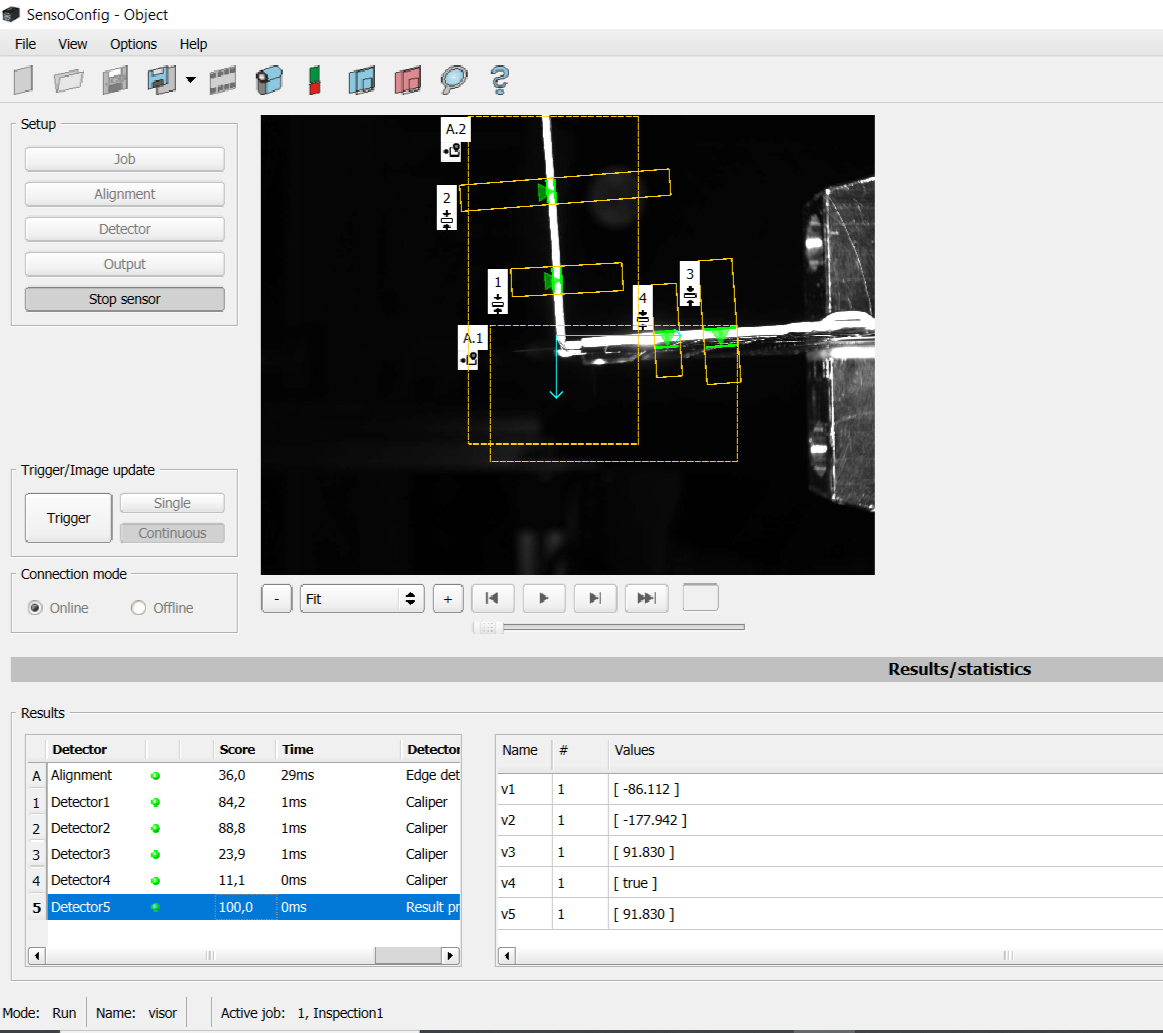
\includegraphics[width=0.6\textwidth]{figures/measurement-detector.png}
    \caption{Detectors in Inspection Camera for angle measurement}
    \label{fig:measurement-detector}
\end{figure}

From the figure \ref{fig:measurement-detector}, the inspection camera uses an alignment detector, four caliper detectors and one results processing of caliper detectors to calculate the angle.
\textbf{Alignment} detector uses a reference detection in the image and aligns the other detectors \textit{w.r.t.} \textbf{Alignment} detector. 
Four \textbf{Detector Caliper} are used to measure the distance between the edges when the detector transitions from dark to light and again from light to dark. Thus two probes, antiparallel setup is used. Angle measurement is of interest, so four points are detected on the sheet. 
Now, the fifth detector, \textbf{Result Processing: Math}, is used to first calculate the angle between two points lying on the same edge of sheet \textit{v}1. Similarly, another pair of points are used to get the angle between them \textit{v}2. Finally, the angle between these \textit{v}1 and \textit{v}2 is calculated to get the final bending angle \textit{v}3. \textit{v}4 is calculated by checking if the angle is within the tolerances. \textit{v}5 is set to \textit{v}3 if the output of \textit{v}4 is true, otherwise it is set to 0. The \hyperref[acro:PLC]{PLC} receives the output \textit{v}4 and \textit{v}5 of detector number 5, \textbf{Result Processing}.
